%------------------------------------------------
%	PACKAGES AND THEMES
%------------------------------------------------

% this is a 4:3 layout.
\documentclass{beamer}
% for 16:9 use this command:
% \documentclass[aspectratio=169]{beamer}

\mode<presentation> {
\usetheme{metropolis}
\setbeamertemplate{caption}[numbered]
\setbeamertemplate{navigation symbols}{} % hide navigation symbols
}

\usepackage{graphicx} % images
\usepackage{algorithm2e}
\usepackage{mathtools}
\DeclarePairedDelimiter{\ceil}{\lceil}{\rceil}
\usepackage{algpseudocode}
\usepackage{booktabs} % allows the use of \toprule, \midrule and \bottomrule in tables
\usepackage[ngerman]{babel}
\usepackage[utf8]{inputenc}
\usepackage[T1]{fontenc}
\usepackage{mathtools}
\usepackage{xcolor}
\usepackage{listings} % code
\usepackage{pgf,tikz} % drawing
\usepackage{pifont} % new symbols
\usepackage{hyperref} % pretty links
% \usepackage{algorithmicx}
% \usepackage{algpseudocode}
% \usepackage[linesnumbered,ruled]{algorithm2e}

% for code keywords within the text
\usepackage{xcolor}
\definecolor{light-gray}{gray}{0.95}
\newcommand{\code}[1]{\colorbox{light-gray}{\texttt{#1}}}

\usepackage{lmodern}
\usepackage{subcaption}
\usepackage{textcomp}
% \usepackage{array}
% \usepackage{longtable}
% \usepackage{verbatim}
%\usepackage{tabularx}
\captionsetup[figure]{font=footnotesize}

\usepackage{amsmath}
\usepackage{amssymb}
\usepackage{amsthm}
% \usepackage{comment}
% \usepackage{enumitem}
% \usepackage[binary-units=true]{siunitx}
% \usepackage{thmtools}
\usepackage{csquotes}
\usepackage{tikz}
\usepackage{float}
\usetikzlibrary{automata,positioning}

% color settings for links
\hypersetup{
    colorlinks=true,
    urlcolor=blue,
    linkcolor=black,
    citecolor=green!50!black
}

\definecolor{mygreen}{RGB}{1,135,1}

\newcommand{\cmark}{\ding{51}}  % checkmark
\newcommand{\xmark}{\ding{55}}  % xmark
\newcommand\scalemath[2]{\scalebox{#1}{\mbox{\ensuremath{\displaystyle #2}}}}

\newcommand{\specialcell}[2][c]{%
  \begin{tabular}[#1]{@{}c@{}}#2\end{tabular}}

\setbeamerfont{bibliography item}{size=\footnotesize}
\setbeamerfont{bibliography entry author}{size=\footnotesize}
\setbeamerfont{bibliography entry title}{size=\footnotesize}
\setbeamerfont{bibliography entry location}{size=\footnotesize}
\setbeamerfont{bibliography entry note}{size=\footnotesize}

% \useoutertheme{miniframes} % navigation design
\useinnertheme{circles} % use non shiny circles (itemize, etc.)

% Main slide colors
% dunkel, hell, mittel
% \definecolor{pale}{RGB}{232, 236, 237}
% \definecolor{prim}{RGB}{53, 109, 120}
% \definecolor{sec}{RGB}{104, 170, 183}
% \definecolor{tert}{RGB}{109, 155, 168}
% \definecolor{quat}{RGB}{9, 59, 68}

\definecolor{pale}{RGB}{255, 255, 255}
% \definecolor{prim}{RGB}{153, 194, 173}
% good: \definecolor{prim}{RGB}{27, 33, 42}
\definecolor{prim}{RGB}{32, 43, 50}
\definecolor{sec}{RGB}{217, 232, 224}
\definecolor{tert}{RGB}{0, 82, 41}
% save
\definecolor{quat}{RGB}{0, 82, 41}

\setbeamercolor{palette primary}{bg=prim,fg=pale}
\setbeamercolor{palette secondary}{bg=sec,fg=pale}
\setbeamercolor{palette tertiary}{bg=tert,fg=pale}
\setbeamercolor{palette quaternary}{bg=quat,fg=pale}
\setbeamercolor{structure}{fg=prim} % itemize, enumerate, etc
\setbeamercolor{section in toc}{fg=prim} % TOC sections

% Block colors
\definecolor{example_color}{RGB}{93, 137, 98}
\definecolor{alert_color}{RGB}{175, 79, 72}

\setbeamercolor{normal text}{fg=prim!20!black,bg=pale!25!white}
\setbeamercolor{alerted text}{fg=alert_color!25!black}
\setbeamercolor{example text}{fg=example_color!25!black}

\setbeamercolor{block title example}{fg=white,bg=example_color}
\setbeamercolor{block body example}{fg=black,bg=example_color!10!white}
\setbeamercolor{block title alerted}{fg=white,bg=alert_color}
\setbeamercolor{block body alerted}{fg=black,bg=alert_color!10!white}

% Override palette coloring
\setbeamercolor{subsection in head/foot}{bg=quat,fg=pale}

\setbeamertemplate{frametitle}{%
    \nointerlineskip%

    \begin{beamercolorbox}[wd=\paperwidth,ht=2.5ex,dp=1ex]{frametitle}
        \hspace*{1ex}\insertframetitle%
        \ifx\insertframesubtitle@empty\else%
        {~\tiny\textcolor{quat!35!black}{\insertframesubtitle}}%
        \fi%
    \end{beamercolorbox}%
}

% math-command for bigger norm
\newcommand\norm[1]{\left\lVert#1\right\rVert}

% use this to include other files
% in this case style definitions for code
% alternative: \include{dateiname}
\lstdefinestyle{latex}{
    language=[LaTeX]TeX,
    inputencoding=utf8,
    basicstyle=\ttfamily,
    keywordstyle=\color{blue!60!black}, % use 60 percent blue and 40 black
    commentstyle=\color{cyan!60!black},
    tabsize=2,
    emph={document,itemize,enumerate,center,tabular,table,
    figure,wrapfigure,minipage,columns,align,bmatrix,
    lstlisting,beamer,frame,tikzpicture},
    emphstyle=\color{magenta!60!black},
    morekeywords={lstset,includegraphics,theenumi,labelitemi,column,color,url,href}
}

\lstdefinestyle{inline_latex}{
    language=[LaTeX]TeX,
    inputencoding=utf8,
    basicstyle=\ttfamily,
    resetmargins= true,
    belowcaptionskip=0pt,
    aboveskip=0pt,
    belowskip=0pt,
    keywordstyle=\color{blue!60!black},
    commentstyle=\color{cyan!60!black},
    emph={document,itemize,enumerate,center,tabular,table,
    figure,wrapfigure,minipage,columns,align,bmatrix,
    lstlisting,beamer,frame,tikzpicture,Parameter},
    emphstyle=\color{magenta!60!black},
    morekeywords={lstset,includegraphics,theenumi,labelitemi,column,color,url,href,Befehlsname}
}

\lstdefinestyle{cpp}{
    language=C++,
    basicstyle=\ttfamily,
    keywordstyle=\color{blue!90!black},
    stringstyle=\color{magenta!60!black},
    commentstyle=\color{green!35!black},
    morecomment=[l][\color{gray!60!black}]{\#},
    tabsize=2
}

\lstdefinestyle{empty}{
    basicstyle=\rmfamily,
    keywordstyle=\bfseries,
    commentstyle=\color{black}\itshape
}

\lstset{style=latex}

%------------------------------------------------
%	TITLE PAGE
%------------------------------------------------

\selectlanguage{ngerman}
\title[]{Execution Monitoring for Long-Term Autonomous Plant Observation with a Mobile Robot}

\author{Tim Bohne}
\institute[]
{
\textit{AG Knowledge-Based Systems}\newline
\textit{DFKI Plan-Based Robot Control Group}
\medskip
}
\date{\today}

% make slide at the beginnig of each section
\AtBeginSection[]{
{\setbeamercolor{background canvas}{bg=white}}}

% where images are locatied
\graphicspath{{./images/}}

\begin{document}

\begin{frame}[plain] % plain slides dont have navigation bars etc.
\titlepage % Print the title page as the first slide
\end{frame}

\begin{frame}
\frametitle{Übersicht} % table of contents slide
\tableofcontents
\end{frame}

% %------------------------------------------------
% \section{Motivation}
% %------------------------------------------------

\begin{frame}
  \frametitle{Langzeit-Autonome Mobile Roboter}
  \textbf{Langzeit}\newline
  \begin{figure}[H]
    \centering
    \begin{subfigure}[b]{0.32\textwidth}
      \centering
      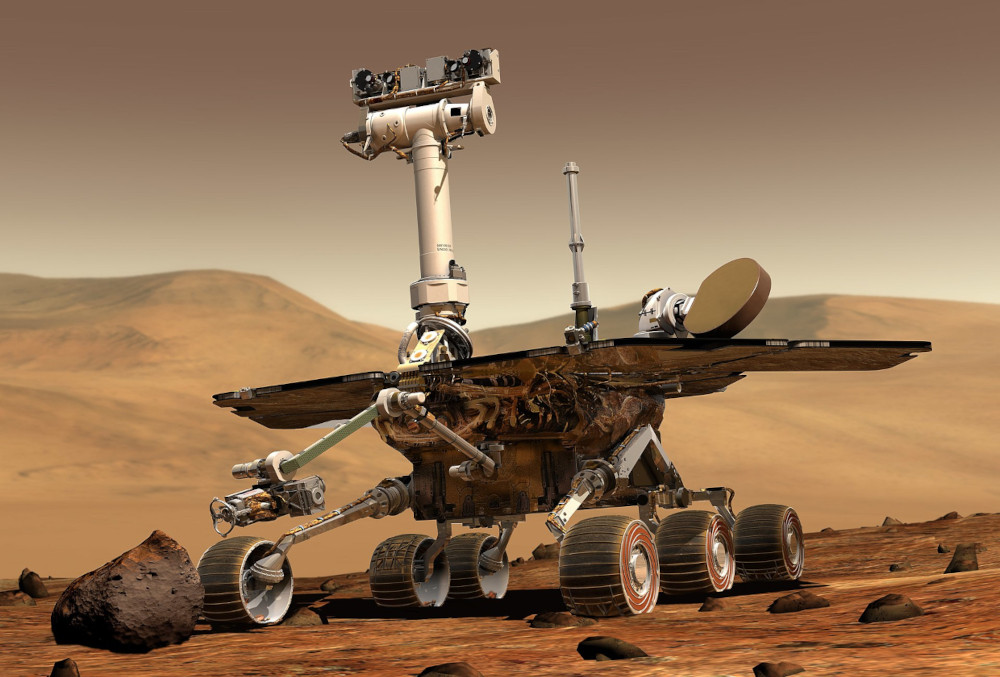
\includegraphics[width=\textwidth]{img/mars_rover.jpg}
      \caption*{$\approx$ Jahre \cite{MarsRover}}
    \end{subfigure}
    \begin{subfigure}[b]{0.32\textwidth}
      \centering
      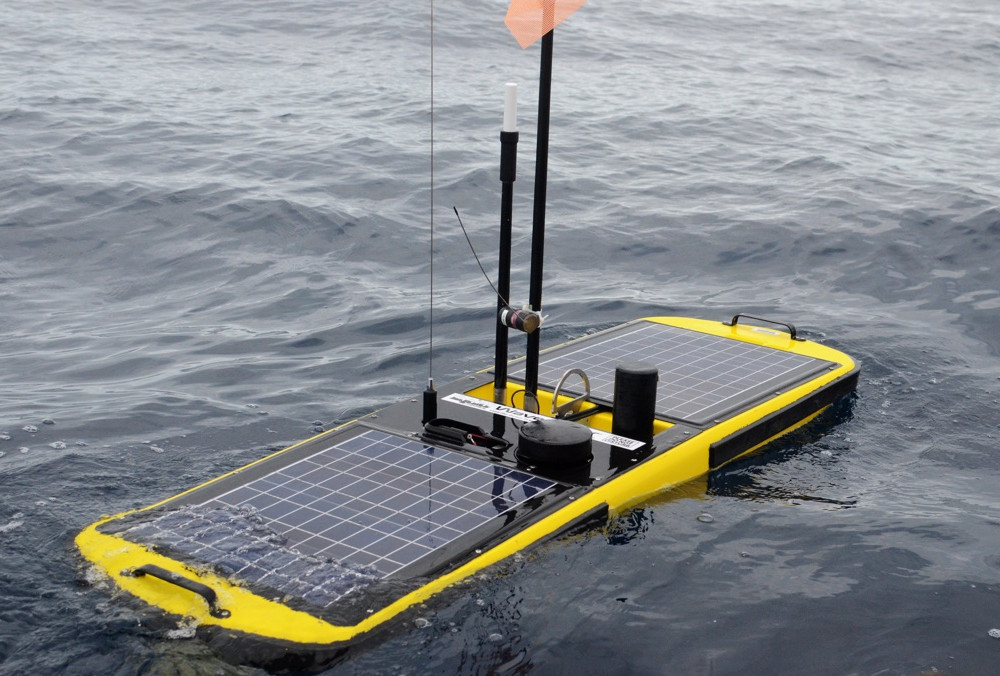
\includegraphics[width=\textwidth]{img/waveglider.jpg}
      \caption*{$\approx$ Monate \cite{WaveGlider}}
    \end{subfigure}
    \begin{subfigure}[b]{0.32\textwidth}
      \centering
      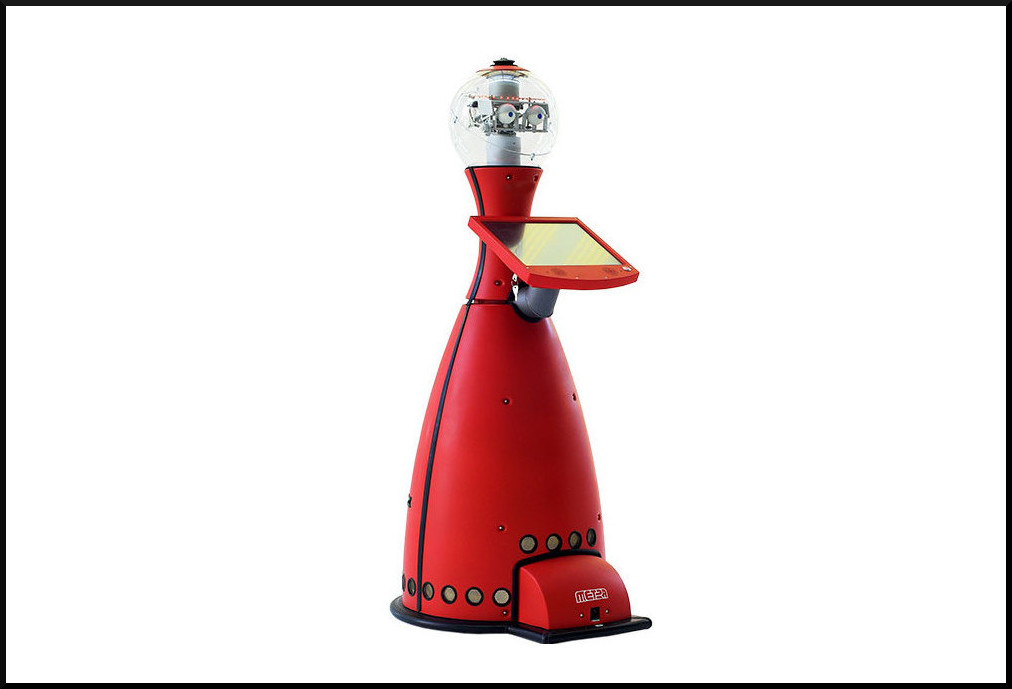
\includegraphics[width=\textwidth]{img/service_robot.jpg}
      \caption*{$\approx$ Wochen \cite{ServiceRobot}}
    \end{subfigure}
  \end{figure}
  \begin{itemize}
    \item Keine strikte Definition \textrightarrow \thinspace \textbf{kontextabhängig}
    \item Hier:
    \begin{itemize}
      \item \textbf{Ladezyklus} - zeitlicher Handlungsradius des Roboters
      \item \textbf{Missionszyklus} - repetitiver Charakter der Mission
    \end{itemize}
    \item \textbf{LB}: Prozesse, die eine Reihe solcher Zyklen erfordern
    \item \textbf{UB}: Wartungsintervalle
  \end{itemize}
\end{frame}

\begin{frame}
  \frametitle{Langzeit-Autonome Mobile Roboter}
  \textbf{Autonomie}
  \begin{itemize}
    \item Ebenfalls nicht scharf definiert und \textbf{kontextabhängig}
    \item \textbf{Kooperation} nicht prinzipiell ausgeschlossen
    \item Hier: \textbf{Vollautonom} - Inanspruchnahme menschlicher Hilfe ausschließlich im Fehlerfall
  \end{itemize}
  \begin{figure}[H]
    \centering
    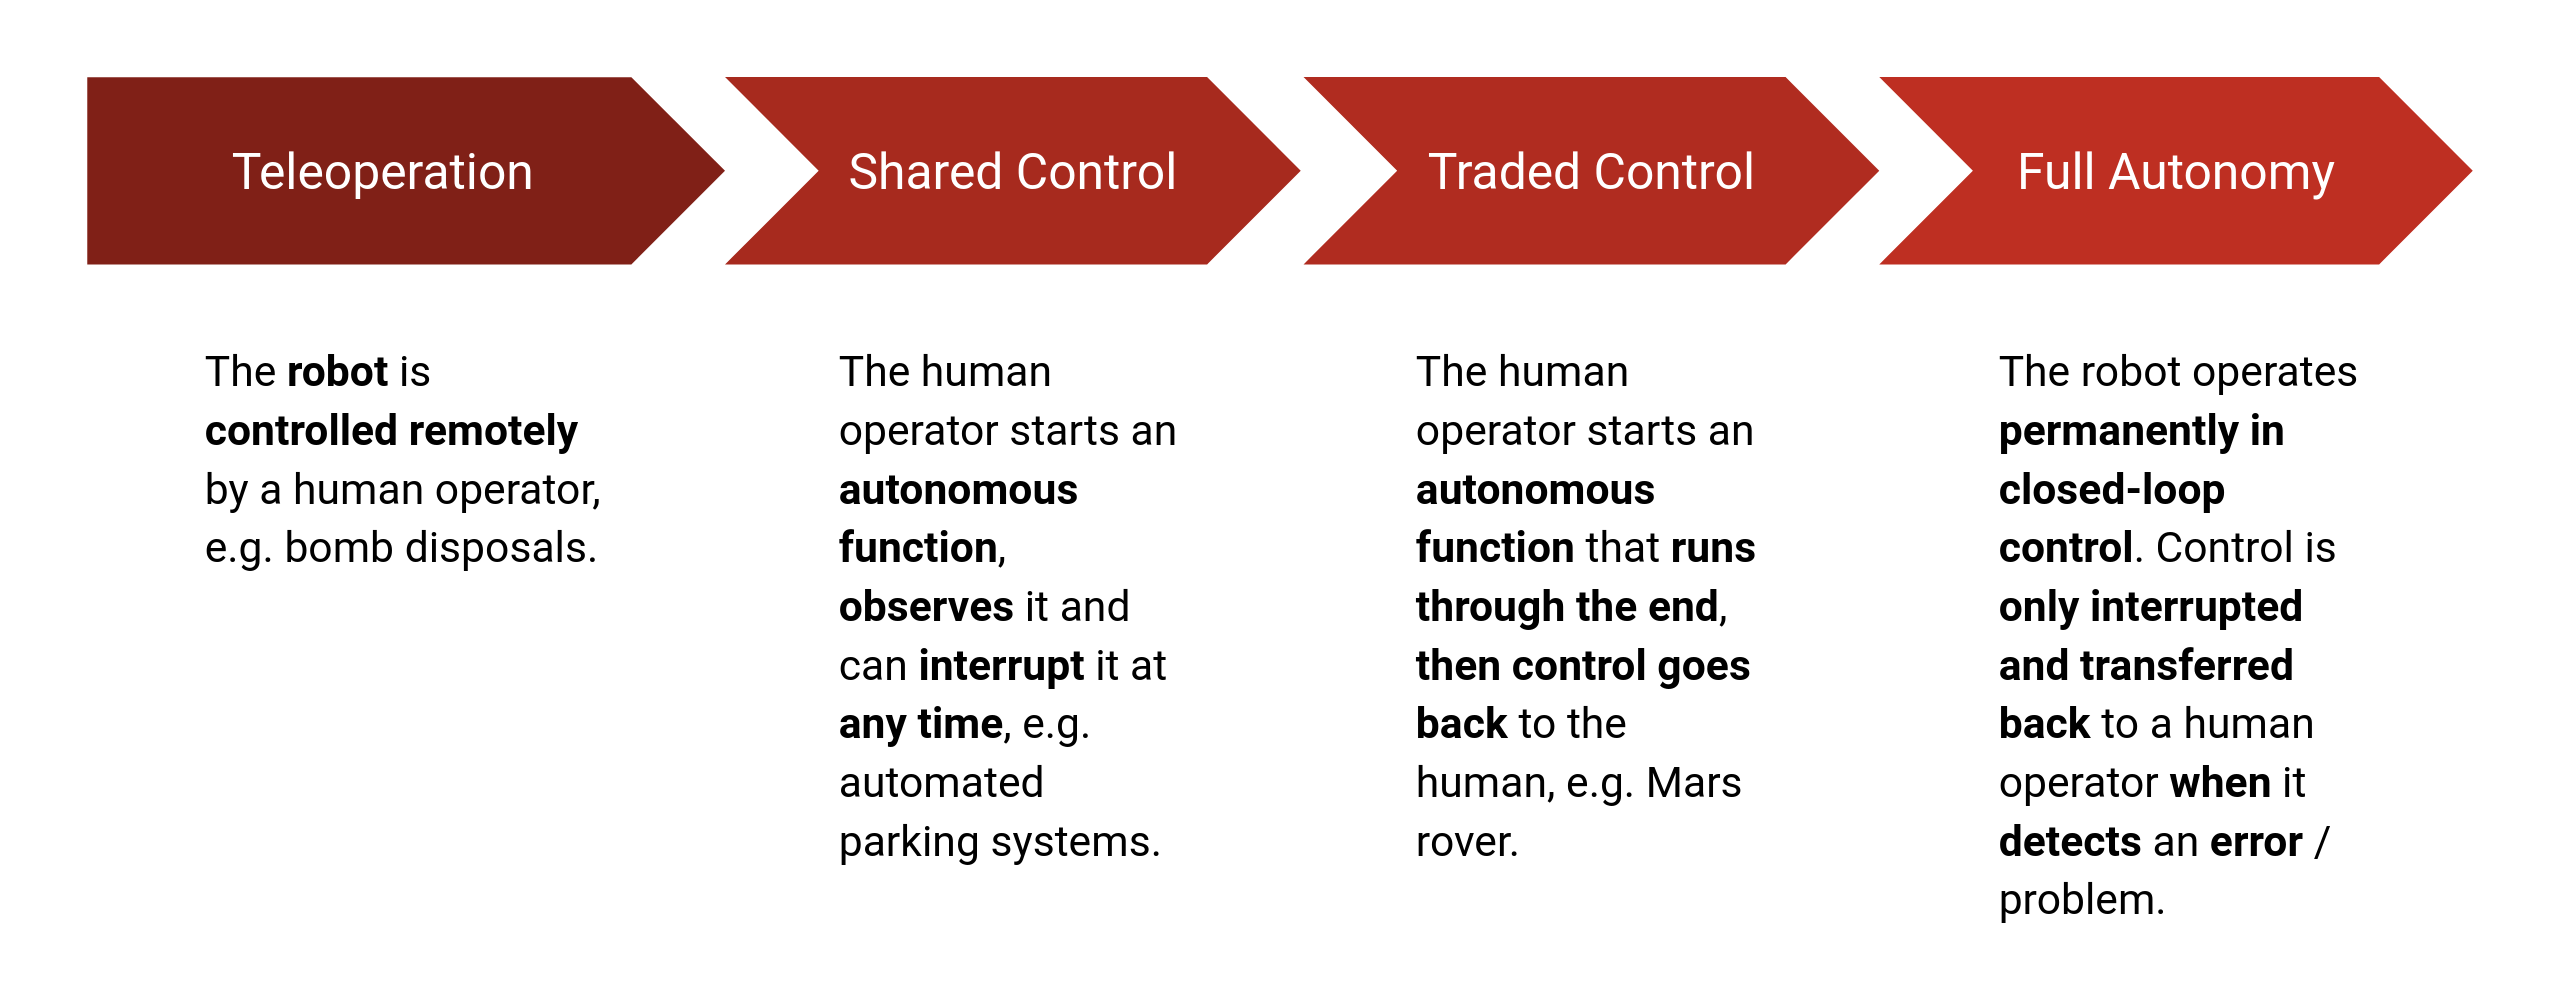
\includegraphics[width=\textwidth]{img/autonomy_spectrum.png}
    \caption*{Spektrum der Autonomie}
  \end{figure}
\end{frame}

\begin{frame}
  \frametitle{Langzeit-Autonome Mobile Roboter}
  \textbf{Mobil}\newline
  System, das in der Lage ist, sich innerhalb bestimmter Grenzen frei in einer Umgebung zu bewegen.
\end{frame}

\begin{frame}
  \frametitle{AROX - Autonomous Robotic Experimentation Platform}
  \begin{figure}[H]
    \centering
    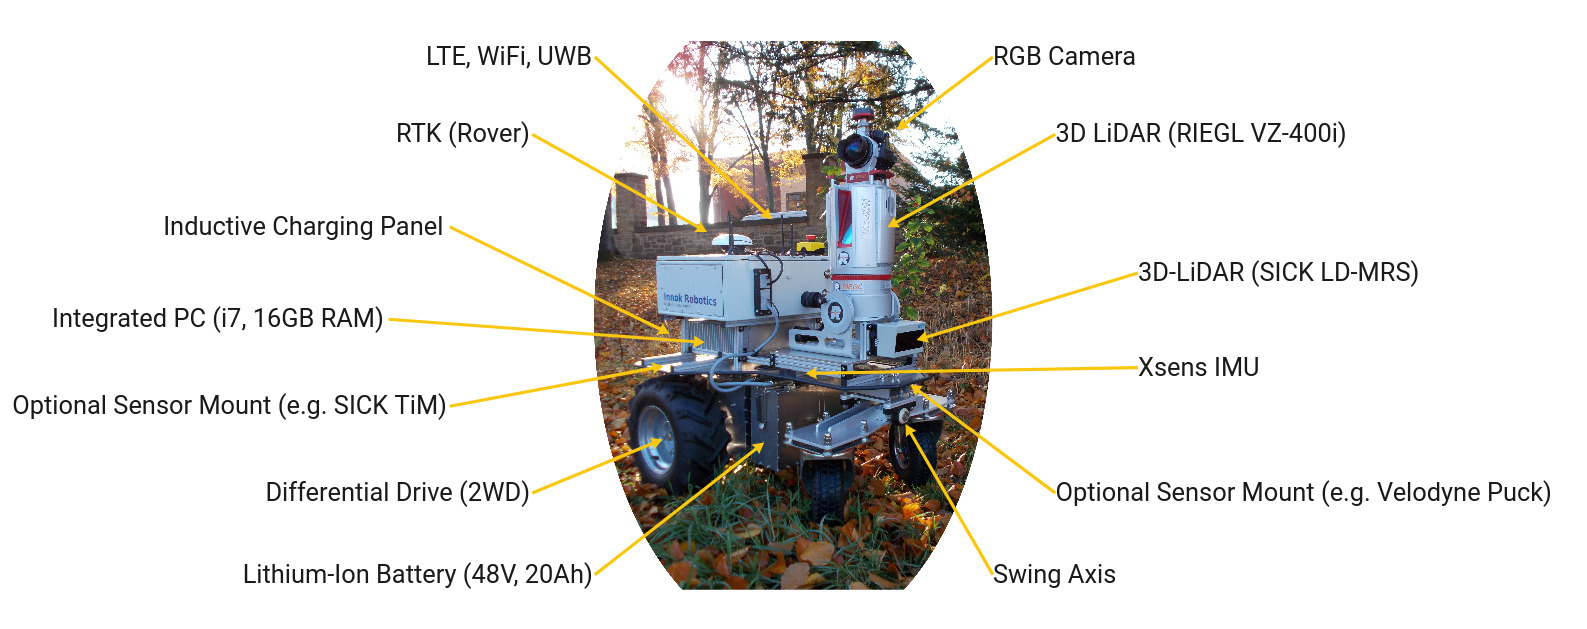
\includegraphics[width=\textwidth]{img/AROX.jpg}
    \caption*{}
  \end{figure}
  \begin{itemize}
    \item \textbf{Lokalisierung}: \code{robot\_localization} \cite{Moore:2014}\newline \textrightarrow \thinspace Sensorfusion von IMU-, Odometrie- und RTK-GNSS-Daten
    \item \textbf{Navigation}: \code{move\_base\_flex} \cite{Puetz:2018}
  \end{itemize}
\end{frame}

\begin{frame}
  \frametitle{Szenario in der Simulation}
  \begin{figure}[H]
    \centering
    \begin{subfigure}[b]{0.49\textwidth}
      \centering
      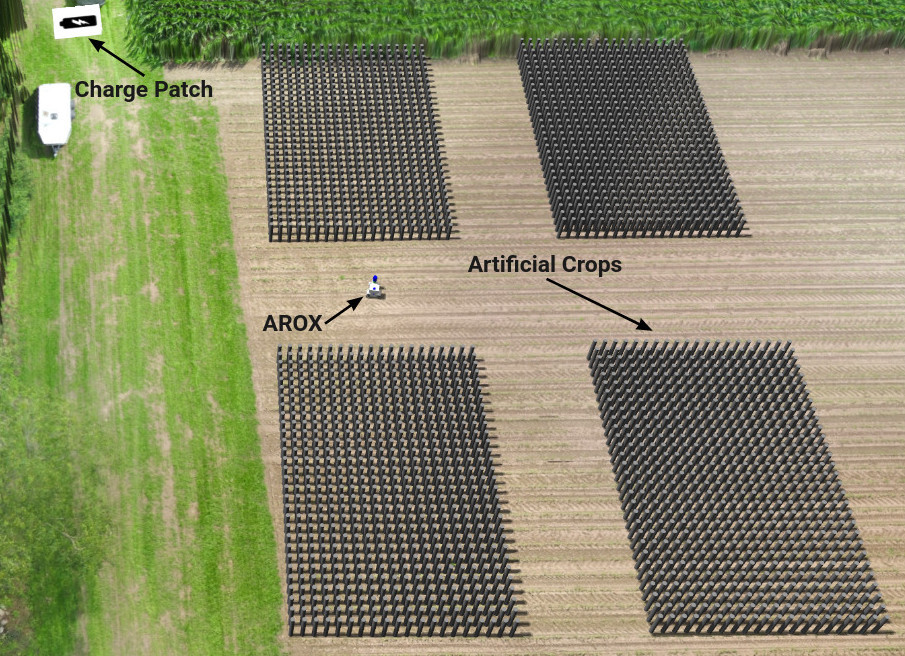
\includegraphics[width=\textwidth]{img/prototype_scenario.jpg}
      \caption*{Prototypisches Layout}
    \end{subfigure}
    \begin{subfigure}[b]{0.49\textwidth}
      \centering
      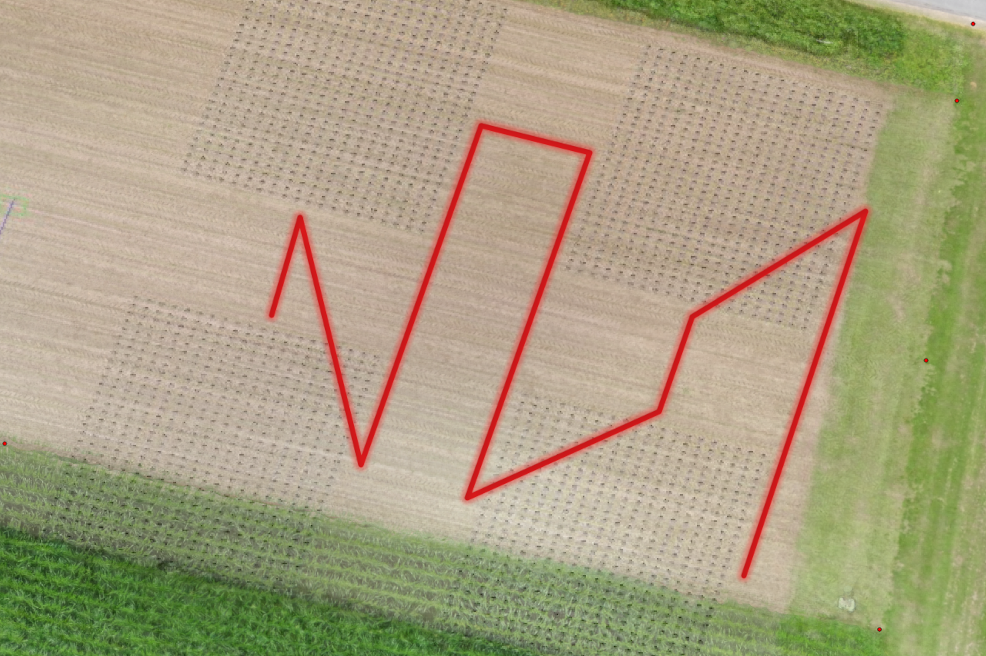
\includegraphics[width=\textwidth]{img/example_path.png}
      \caption*{Beisiel Scan-Route}
    \end{subfigure}
  \end{figure}
  \begin{itemize}
    \item 3D-Lidar-Scans / Hyperspektralaufnahmen von Pflanzen \textrightarrow \thinspace Wachstumsfortschritt überwachen / Merkmale erkennen
    \item Dynamische, unstrukturierte Umgebung
    \item $2.5D$-Simulation der Testfeld-Umgebung in \textit{Gazebo} inkl. AROX-Modell (URDF)
  \end{itemize}
\end{frame}

\begin{frame}
  \frametitle{Herausforderungen für Langzeitautonomie}
  \textbf{Bedingungen:}
  \begin{enumerate}
    \item Kann im betrachteten Szenario praktisch auftreten
    \item Kann das reibungslose Funktionieren des Systems / die Qualität der Ergebnisse beeinträchtigen
    \item Kann durch Monitoring-Methoden detektiert / gelöst / kommuniziert werden
  \end{enumerate}
\end{frame}

\begin{frame}
  \frametitle{Herausforderungen für Langzeitautonomie}
  \begin{itemize}
    \item \textbf{Energiemanagement}
    \item \textbf{Fehlgeschlagener Ladevorgang}
    \item \textbf{Extreme Wetterbedingungen}
    \item \textbf{Sensorausfall (Wahrnehmung)}
    \item \textbf{Datenmanagement}
    \item \textbf{Verbindungsabbruch}
    \item \textbf{Navigationsfehler}
    \item \textbf{Fehlerhafte / ungenaue Lokalisierung}
    \item \textbf{Planverteilungsfehler}
  \end{itemize}
  \begin{figure}[H]
    \raggedleft
    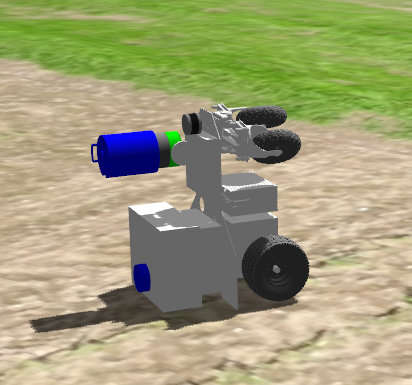
\includegraphics[width=0.3\textwidth]{img/AROX_fall.png}
  \end{figure}
\end{frame}

\begin{frame}
  \frametitle{Herausforderungen für Langzeitautonomie}
  \textbf{Klassifikation:}
  \begin{enumerate}
    \item Roboter detektiert ein Problem und ist in der Lage, es selbstständig zu lösen
    \item Roboter detektiert ein Problem, ist jedoch nicht in der Lage, es zu lösen \textrightarrow \thinspace ruft menschlichen Operator
    \item Roboter hat Störung / Problem, detektiert es jedoch nicht und kann es daher nicht lösen / kommunizieren
  \end{enumerate}
  \textrightarrow \thinspace initial wird jedes potenzielle Problem als Typ $3$ eingestuft
\end{frame}

\begin{frame}
  \frametitle{Abstrakte Architektur autonomer Akteure}
  \begin{figure}[H]
    \centering
    \begin{subfigure}[b]{0.49\textwidth}
        \centering
        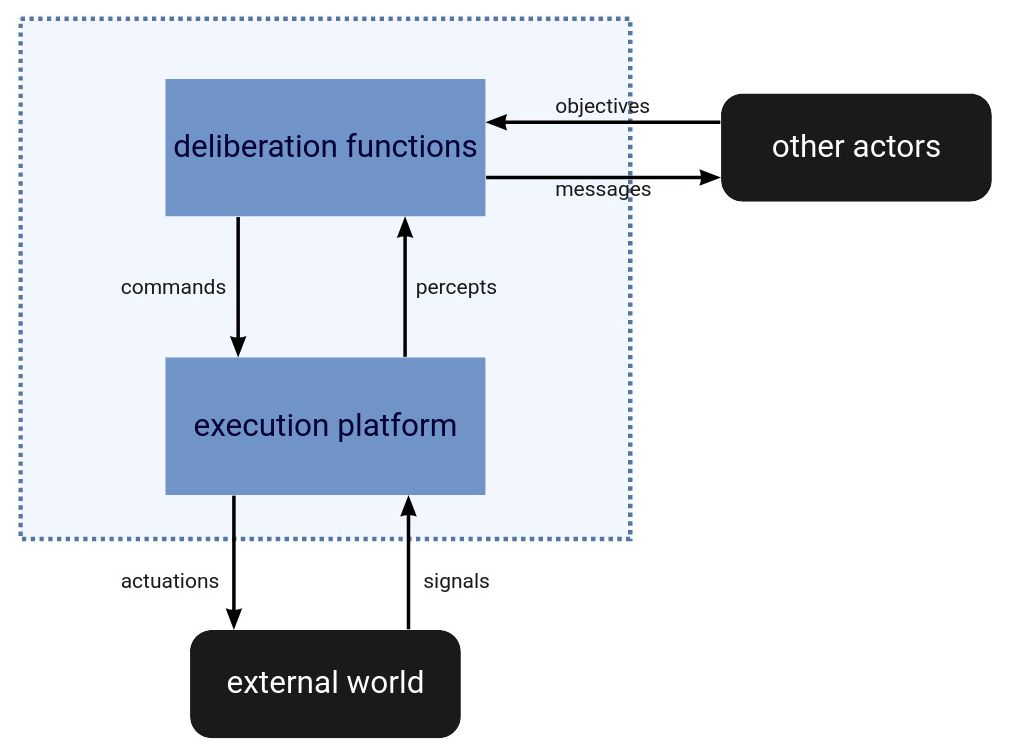
\includegraphics[width=\textwidth]{img/GNT_actor_new.png}
    \end{subfigure}
    \hfill
    \begin{subfigure}[b]{0.49\textwidth}
        \centering
        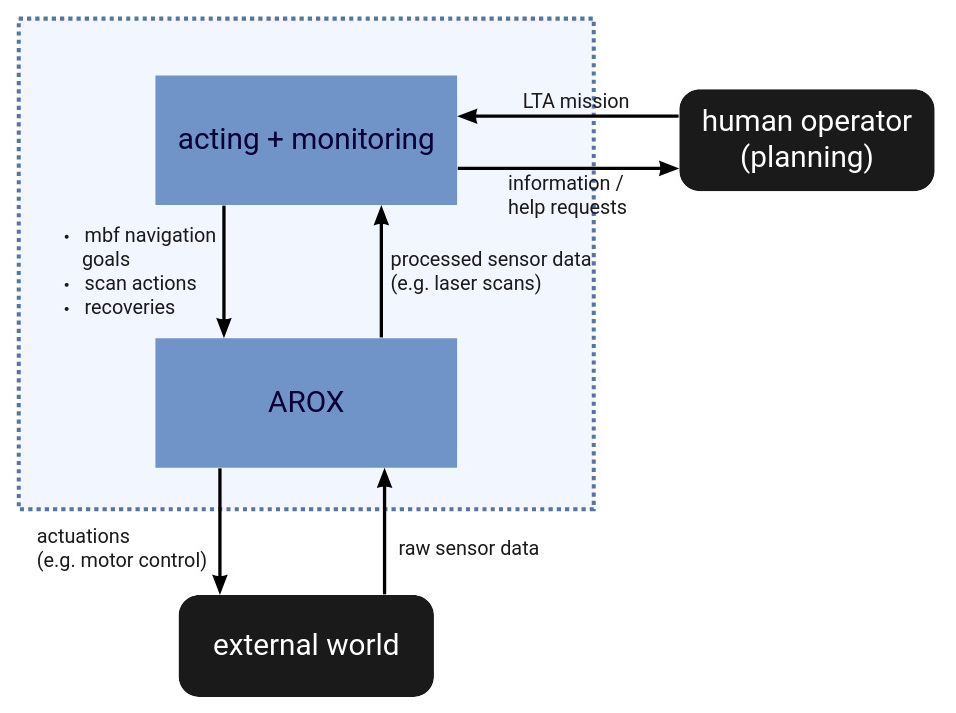
\includegraphics[width=\textwidth]{img/MSC_actor_new.png}
    \end{subfigure}
  \end{figure}
\end{frame}

\begin{frame}
  \frametitle{Execution Monitoring State Machine Architecture}
  Architecture of the Hierarchical State Machine (High-Level)
  \begin{figure}[H]
    \centering
    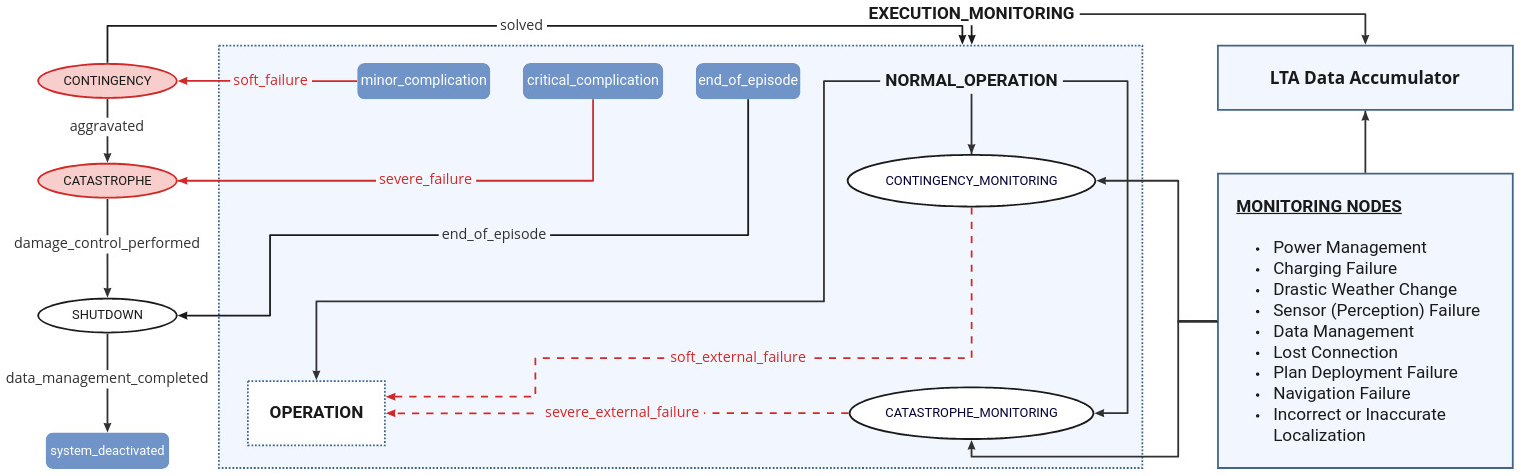
\includegraphics[width=\textwidth]{img/SMACH_high_level.png}
  \end{figure}
\end{frame}

\begin{frame}
  \frametitle{Execution Monitoring State Machine Architecture}
  Architecture of the Embedded State Machine (Low-Level)
  \begin{figure}[H]
    \centering
    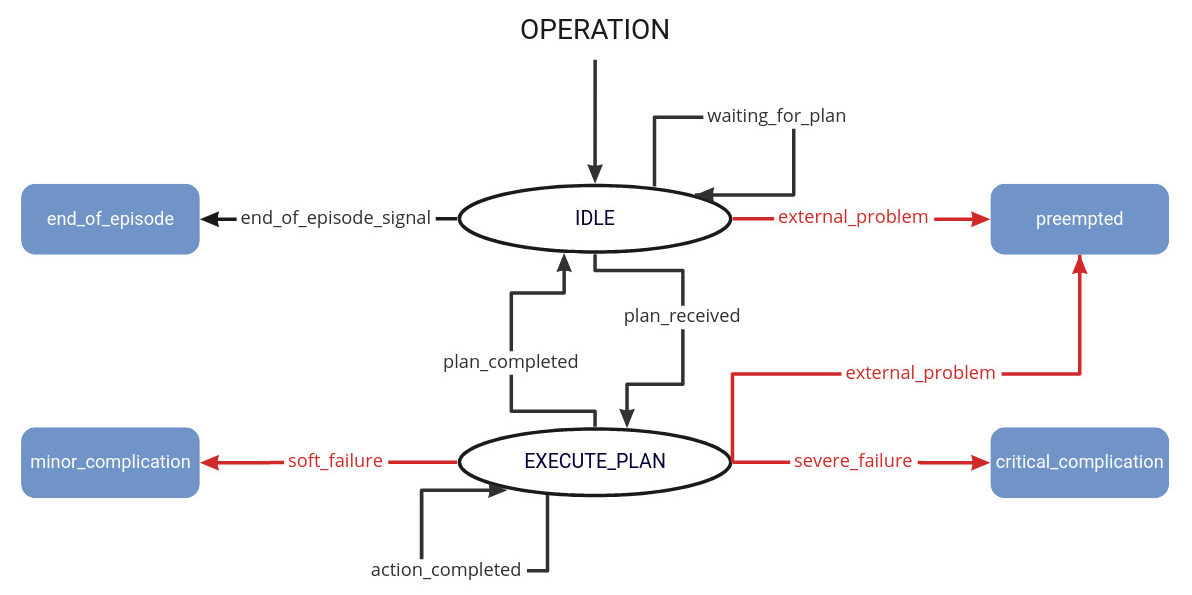
\includegraphics[width=0.8\textwidth]{img/SMACH_low_level.png}
  \end{figure}
\end{frame}

\begin{frame}
  \frametitle{Black Box to Learn from Experience}
  Database Entries Shown in MongoDB Client
  \begin{figure}[H]
    \centering
    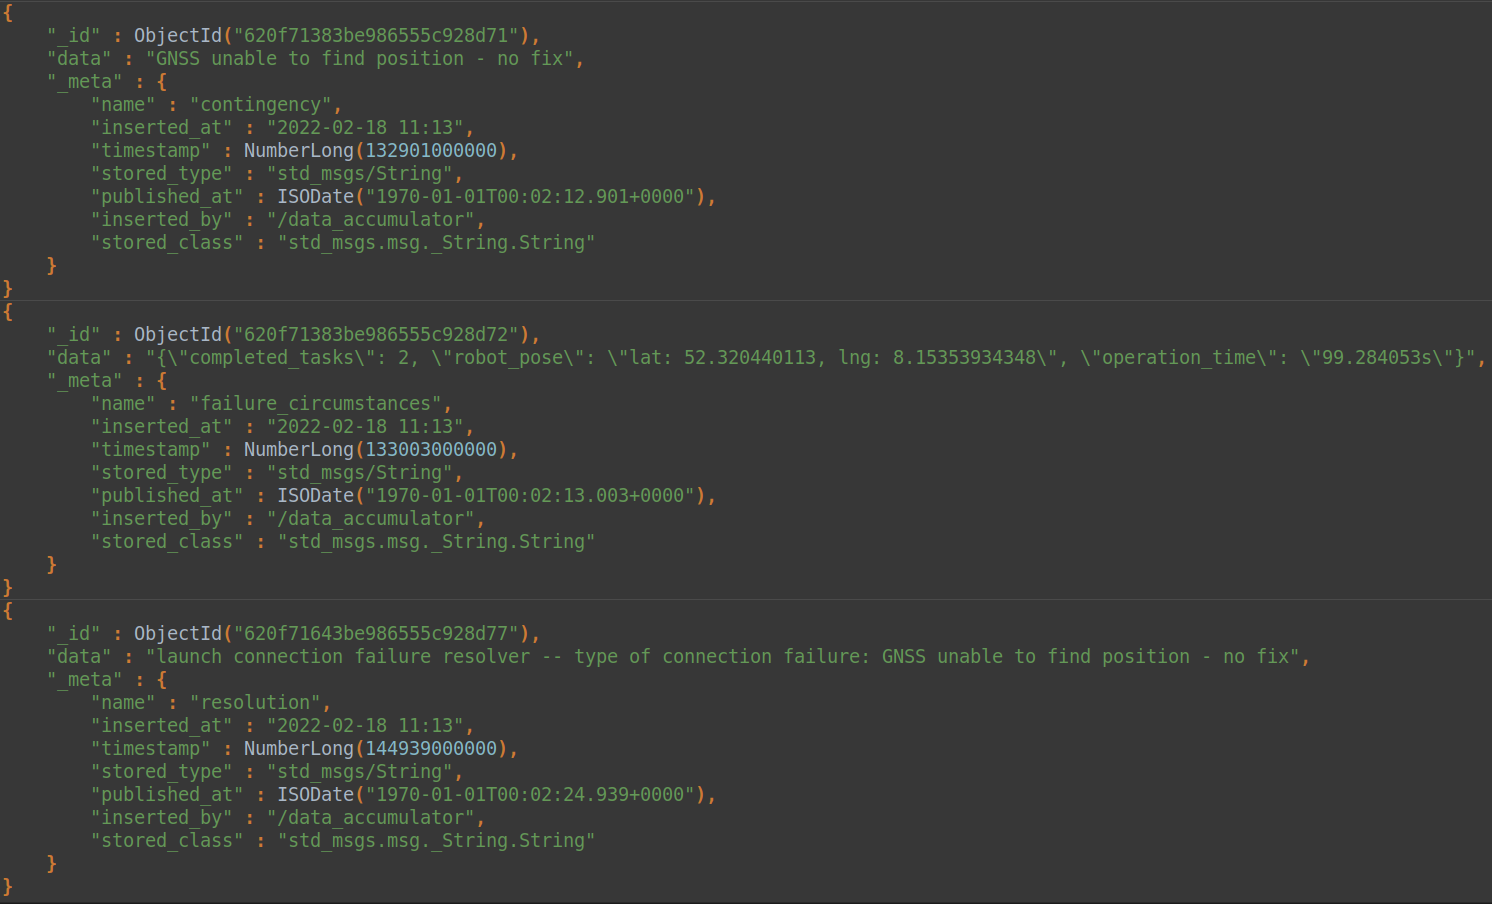
\includegraphics[width=0.8\textwidth]{img/database_entries.png}
  \end{figure}
\end{frame}

\begin{frame}
  \frametitle{Plan Generation and Format}
  \begin{figure}[H]
    \centering
    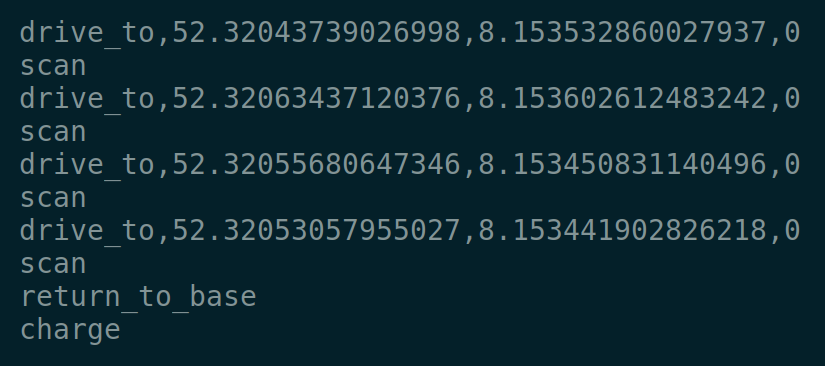
\includegraphics[width=0.4\textwidth]{img/plan_example.png}
  \end{figure}
\end{frame}

\begin{frame}
  \frametitle{Interrupt and Resume Normal Operation}
\end{frame}

\begin{frame}
  \frametitle{Exemplarisch: GNSS Connection Failures}
  \begin{figure}[H]
    \centering
    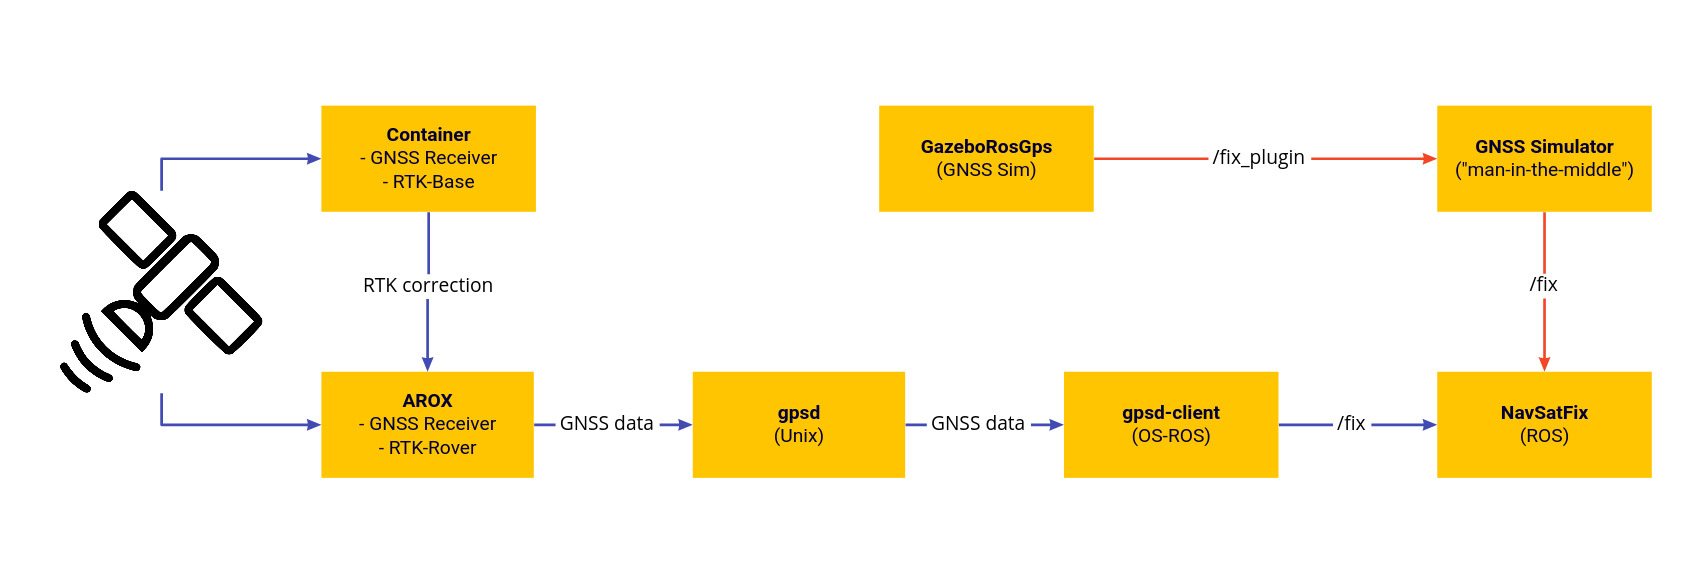
\includegraphics[width=\textwidth]{img/GNSS_comm.png}
  \end{figure}
  \begin{itemize}
    \item \textcolor{blue}{Praxis} / \textcolor{red}{Simulation}
    \item Resultat: \code{NavSatFix}-Daten auf \code{/fix} Topic
  \end{itemize}
\end{frame}

\begin{frame}
  \frametitle{Exemplarisch: GNSS Connection Failures}
  \begin{figure}[H]
    \centering
    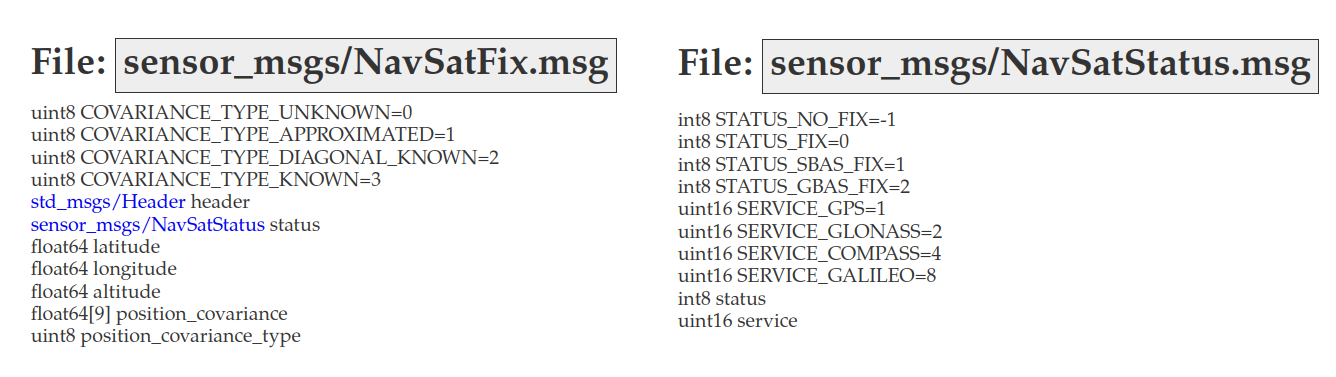
\includegraphics[width=\textwidth]{img/navsatfix.png}
  \end{figure}
  \begin{itemize}
    \item \textbf{Kovarianzmatrix}: $c_{ij} \in C_{3 \times 3}$ with $i, j \in \{E, N, U\}$
    \item \textbf{Standardabweichung} in $m$: $\sqrt{c_{ii}} \thinspace \forall \thinspace i \in \{E, N, U\}$
  \end{itemize}
\end{frame}

\begin{frame}
  \frametitle{Exemplarisch: GNSS Connection Failures}
  \begin{figure}[H]
    \centering
    \begin{subfigure}[b]{0.49\textwidth}
        \centering
        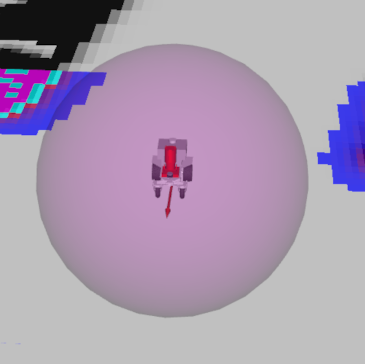
\includegraphics[width=0.75\textwidth]{img/GNSS_cov_low.png}
        \caption{\textsc{Relativ geringe Unsicherheit}}
    \end{subfigure}
    \hfill
    \begin{subfigure}[b]{0.49\textwidth}
        \centering
        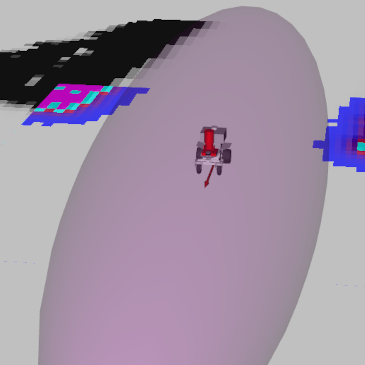
\includegraphics[width=0.75\textwidth]{img/GNSS_cov_high.png}
        \caption{\textsc{Hohe Unsicherheit}}
    \end{subfigure}
    \begin{itemize}
      \item (a): ENU: $(\sqrt{6}m, \sqrt{6}m, \sqrt{6}m)$
      \item (b): ENU: $(\sqrt{101}m, \sqrt{6}m, \sqrt{6}m)$
    \end{itemize}
  \end{figure}
\end{frame}

\begin{frame}
  \frametitle{Exemplarisch: GNSS Connection Failures}
  \textbf{Qualitative Bewertung einer prinzipiell funktionierenden GNSS-Verbindung}
  \begin{itemize}
    \item gut: \code{STATUS\_GBAS\_FIX}, $\geq$ \code{COVARIANCE\_TYPE\_DIAGONAL\_KNOWN}, $\sqrt{c_{ii}} \leq d_{max} \thinspace \forall \thinspace i \in \{E, N, U\}$, $d_{max} \in \mathbb{R}_{0}^{+}$
    \item medium: $\geq$ \code{STATUS\_FIX}, $\geq$ \code{COVARIANCE\_TYPE\_APPROXIMATED}, Standardabweichungen $\leq d_{max}$
    \item schlecht: $\geq$ \code{STATUS\_FIX}, Kovarianztyp unbekannt
    \item Information via \code{/robot\_info}
  \end{itemize}
\end{frame}

\begin{frame}
  \frametitle{Exemplarisch: GNSS Connection Failures}
  \textbf{Problemfall: Nachricht auf \code{/contingency\_preemption}}
  \begin{itemize}
    \item Verbindungsabbruch
    \item Status unzulässig bzw. \code{STATUS\_NO\_FIX}
    \item Längen- und Breitengrad-Informationen nicht vorhanden bzw. unzulässig
    \item Standardabweichungen
    \begin{itemize}
      \item absolute Werte (zulässig / zu groß)
      \item Entwicklung über die Zeit
    \end{itemize}
  \end{itemize}
  \textbf{Lösung}: Kurze Auszeit + erneuter Test, bei wiederholtem Misserfolg Kommunikation des Problems
\end{frame}

\begin{frame}
  \frametitle{Exemplarisch: Navigationsfehler}
  \textbf{Fall 1}: Es existiert ein Pfad, \code{move\_base\_flex} findet ihn jedoch nicht (direkt)
  \begin{figure}[H]
    \centering
    \begin{subfigure}[b]{0.49\textwidth}
        \centering
        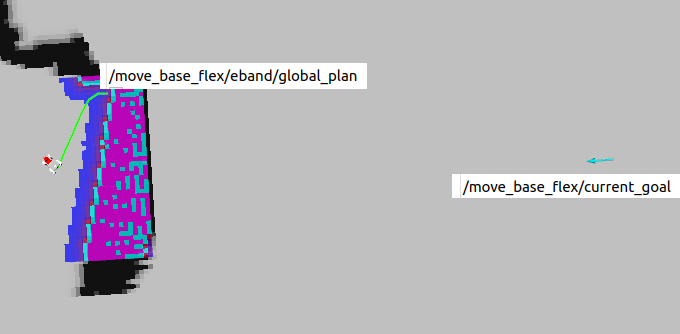
\includegraphics[width=\textwidth]{img/nav_fail_wrong_route_0.png}
        \caption{\code{move\_base\_flex}\textsc{Route (rviz)}}
        \label{fig:nav_fail_rviz}
    \end{subfigure}
    \hfill
    \begin{subfigure}[b]{0.49\textwidth}
        \centering
        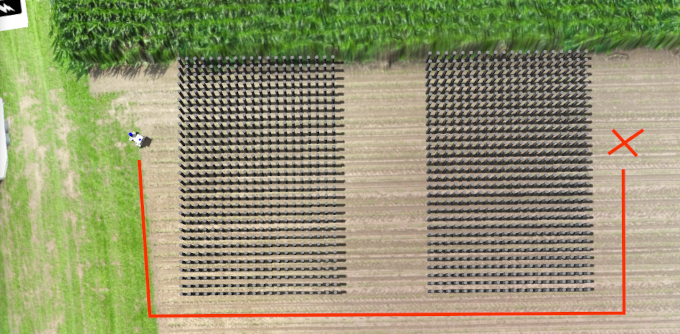
\includegraphics[width=\textwidth]{img/nav_fail_wrong_route_1.png}
        \caption{\textsc{Feasible Route (Gazebo)}}
        \label{fig:nav_fail_gazebo}
    \end{subfigure}
  \end{figure}
\end{frame}

\begin{frame}
  \frametitle{Exemplarisch: Navigationsfehler}
  \textbf{Fall 2}: Es existiert kein Pfad
  \begin{figure}[H]
    \centering
    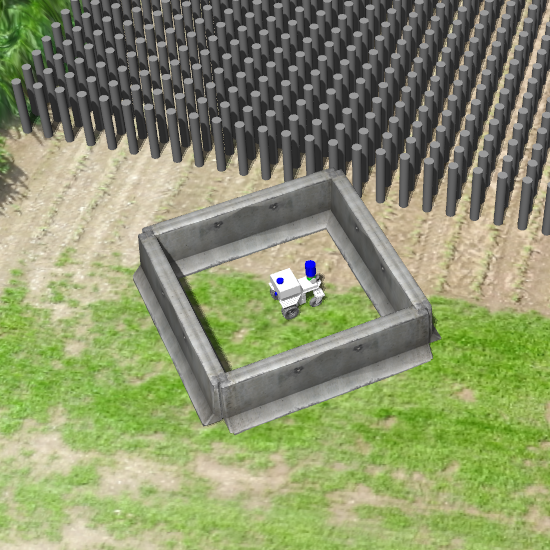
\includegraphics[width=0.3\textwidth]{img/robot_prison.png}
  \end{figure}
\end{frame}

\begin{frame}
  \frametitle{Exemplarisch: Navigationsfehler}
  Simulation statischer Hindernisse
  \begin{figure}[H]
    \centering
    \begin{subfigure}[b]{0.24\textwidth}
        \centering
        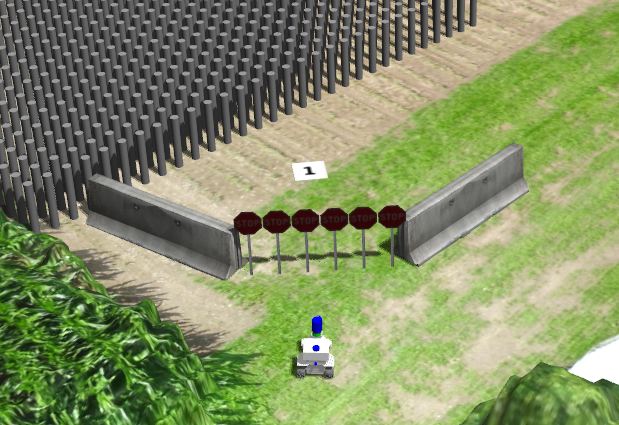
\includegraphics[width=\textwidth]{img/static_1.png}
        \caption{\textsc{Szenario $1$}}
        \label{fig:static_1}
    \end{subfigure}
    \hfill
    \begin{subfigure}[b]{0.24\textwidth}
        \centering
        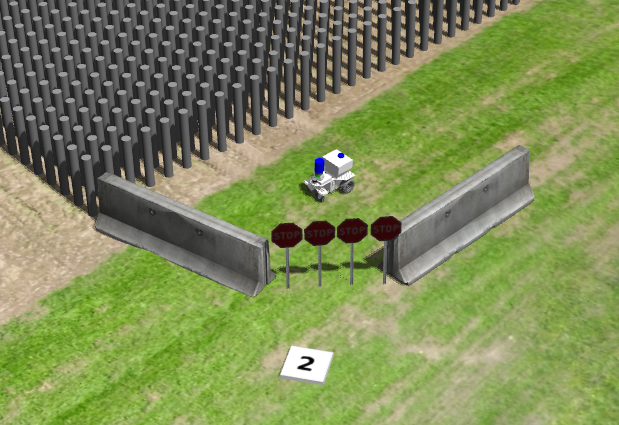
\includegraphics[width=\textwidth]{img/static_2.png}
        \caption{\textsc{Szenario $2$}}
        \label{fig:static_2}
    \end{subfigure}
    \begin{subfigure}[b]{0.24\textwidth}
        \centering
        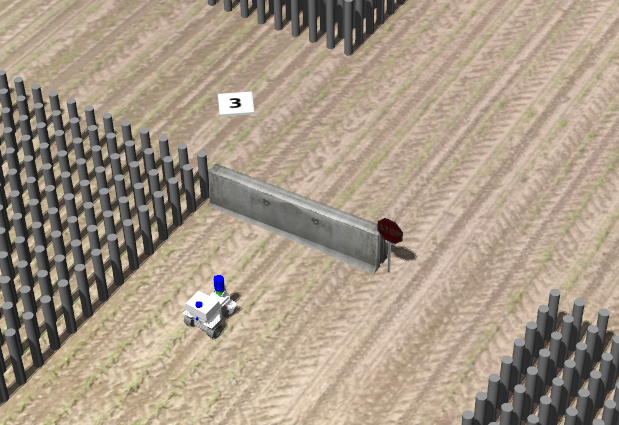
\includegraphics[width=\textwidth]{img/static_3.png}
        \caption{\textsc{Szenario $3$}}
        \label{fig:static_3}
    \end{subfigure}
    \hfill
    \begin{subfigure}[b]{0.24\textwidth}
        \centering
        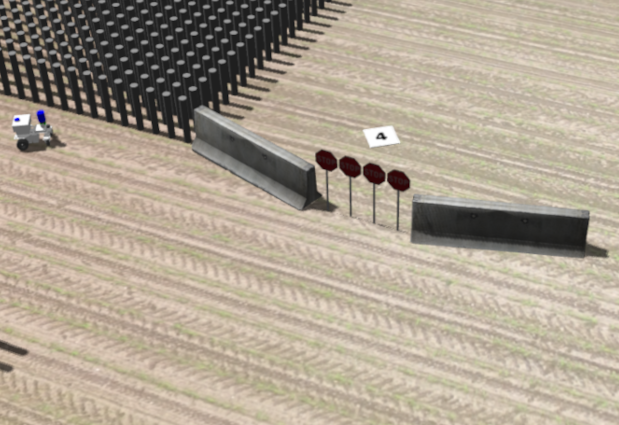
\includegraphics[width=\textwidth]{img/static_4.png}
        \caption{\textsc{Szenario $4$}}
        \label{fig:static_4}
    \end{subfigure}
  \end{figure}
  \begin{figure}[H]
    \centering
    \begin{subfigure}[b]{0.24\textwidth}
        \centering
        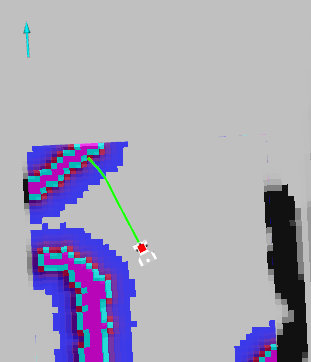
\includegraphics[width=\textwidth]{img/succ_1.png}
        \caption{\textsc{}}
        \label{fig:succ_1}
    \end{subfigure}
    \hfill
    \begin{subfigure}[b]{0.24\textwidth}
        \centering
        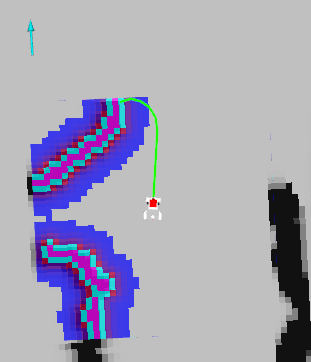
\includegraphics[width=\textwidth]{img/succ_2.png}
        \caption{\textsc{}}
        \label{fig:succ_2}
    \end{subfigure}
    \begin{subfigure}[b]{0.24\textwidth}
        \centering
        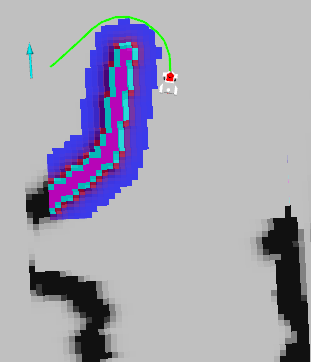
\includegraphics[width=\textwidth]{img/succ_3.png}
        \caption{\textsc{}}
        \label{fig:succ_3}
    \end{subfigure}
    \hfill
    \begin{subfigure}[b]{0.24\textwidth}
        \centering
        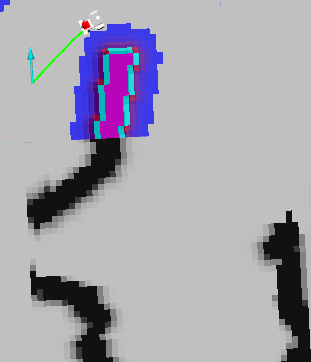
\includegraphics[width=\textwidth]{img/succ_4.png}
        \caption{\textsc{}}
        \label{fig:succ_4}
    \end{subfigure}
  \end{figure}
\end{frame}

\begin{frame}
  \frametitle{Klassifikation der Probleme in Bezug auf ihren potenziellen Schaden}
  \begin{figure}[H]
    \centering
    \resizebox{\textwidth}{!}{
    \begin{tabular}{| c | c | c | c | c |}
        \hline
        \textbf{problem} & \specialcell{\textbf{contingency} \\ \small{\textit{(no contingencies without monitoring)}} \\ sim + prac} & \specialcell{\textbf{catastrophe} \\ \small{\textit{((\cmark) \textrightarrow indirectly)}} \\ sim \quad\quad\quad\quad prac} & \specialcell{\textbf{potential to render mission worthless} \\ sim \quad\quad\quad\quad prac} \\ \hline
        power\_management & \cmark & \cmark \quad\quad\quad\quad\quad \cmark & \cmark \quad\quad\quad\quad\quad \cmark \\ \hline
        charging\_failure & \cmark & \cmark \quad\quad\quad\quad\quad \cmark & \cmark \quad\quad\quad\quad\quad \cmark \\ \hline
        drastic\_weather\_change & \cmark & \thinspace\thinspace \xmark \quad\quad\quad\quad\quad (\cmark) & \xmark \quad\quad\quad\quad\quad \cmark \\ \hline
        sensor\_failure & \cmark & \xmark \thinspace\thinspace\quad\quad\quad\quad\quad \xmark & \cmark \quad\quad\quad\quad\quad \cmark \\ \hline
        data\_management & \cmark & \xmark \thinspace\thinspace\quad\quad\quad\quad\quad \xmark & \cmark \quad\quad\quad\quad\quad \cmark \\ \hline
        lost\_connection & \cmark & (\cmark) \quad\quad\quad\quad (\cmark) & \cmark \quad\quad\quad\quad\quad \cmark \\ \hline
        plan\_deployment\_failure & \cmark & (\cmark) \quad\quad\quad\quad (\cmark) & \cmark \quad\quad\quad\quad\quad \cmark \\ \hline
        navigation\_failure & \cmark & (\cmark) \quad\quad\quad\quad (\cmark) & \cmark \quad\quad\quad\quad\quad \cmark \\ \hline
        incorrect\_localization & \cmark & (\cmark) \quad\quad\quad\quad (\cmark) & \cmark \quad\quad\quad\quad\quad \cmark \\ \hline
    \end{tabular}}
  \end{figure}
\end{frame}

\begin{frame}
  \frametitle{Fallback Solution - Requesting Help of a Human Operator}
\end{frame}



% % %------------------------------------------------
% % \section{Graph Neural Networks (GNNs)}
% % %------------------------------------------------

% %------------------------------------------------
% \section{Robustheit}
% %------------------------------------------------

% %------------------------------------------------
% \subsection{GNNs: Manipulation der Knoten-Attribute}
% %------------------------------------------------

% %------------------------------------------------
% \subsection{GNNs: Manipulation der Graph-Struktur}
% %------------------------------------------------

% %------------------------------------------------
% \section{Fazit / Ausblick}
% %------------------------------------------------

\begin{frame}[allowframebreaks]
  \bibliographystyle{plain}
  \bibliography{sources.bib}
\end{frame}

\end{document}
